\documentclass{article}

% content/resources/templates/preamble.tex
\usepackage[margin=0.6in]{geometry}
\author{Milav Dabgar}
\usepackage{amsmath,amssymb,amsthm}
\usepackage{booktabs}
\usepackage{multirow}
\usepackage{xcolor}
\usepackage{tcolorbox}
\tcbuselibrary{breakable,skins}
\usepackage[colorlinks=true,linkcolor=blue]{hyperref}
\usepackage{titlesec}
\usepackage{enumitem}
\usepackage{tikz}
\usepackage{pgfplots}
\usepackage{circuitikz}
\usepackage[version=4]{mhchem}
\usepackage{longtable}
\usepackage{array}
\usepackage{float}
\usepackage{caption}
\usepackage{listings}

\lstset{
  basicstyle=\small\ttfamily,
  breaklines=true,
  breakatwhitespace=false,
  postbreak=\mbox{\textcolor{red}{$\hookrightarrow$}\space},
  float=false,
  numbers=left,
  numberstyle=\tiny\color{gray},
  numbersep=10pt,
  xleftmargin=2em,
  keywordstyle=\color{blue},
  commentstyle=\color{green!60!black},
  stringstyle=\color{purple},
  backgroundcolor=\color{gray!5},
  showstringspaces=false,
  tabsize=2,
  captionpos=b,
  keepspaces=true,
  columns=flexible
}

\pgfplotsset{compat=1.18}
\usetikzlibrary{shapes,arrows,positioning,calc,patterns,decorations.pathmorphing,decorations.markings,arrows.meta}

% Color scheme
\definecolor{headcolor}{RGB}{0,102,204}
\definecolor{keycolor}{RGB}{220,20,60}
\definecolor{solutioncolor}{RGB}{34,139,34}
\definecolor{mnemoniccolor}{RGB}{148,0,211}
\definecolor{codecolor}{RGB}{0,0,100}

% Spacing
\setlength{\parskip}{3pt}
\setlist[itemize]{nosep}
\setlist[enumerate]{nosep}

% Title formatting
\titleformat{\section}{\Large\bfseries\color{headcolor}}{\thesection}{1em}{}
\titleformat{\subsection}{\large\bfseries\color{headcolor}}{\thesubsection}{1em}{}

% Pandoc tightlist compatibility
\providecommand{\tightlist}{%
  \setlength{\itemsep}{0pt}\setlength{\parskip}{0pt}}

% Pandoc longtable compatibility
\newcounter{none}
\def\thenone{}


% content/resources/templates/english-boxes.tex

% Custom environments
\newtcolorbox{solutionbox}{
 breakable,
 enhanced,
 colback=solutioncolor!5!white,
 colframe=solutioncolor!75!black,
 fonttitle=\bfseries,
 title=Solution
}

\newtcolorbox{solutionboxnobreak}{
 colback=solutioncolor!5!white,
 colframe=solutioncolor!75!black,
 fonttitle=\bfseries,
 title=Solution
}

\newtcolorbox{keyformula}{
 breakable,
 enhanced,
 colback=keycolor!5!white,
 colframe=keycolor!75!black,
 fonttitle=\bfseries,
 title=Key Formula
}

\newtcolorbox{mnemonicboxenv}{
 breakable,
 enhanced,
 colback=mnemoniccolor!5!white,
 colframe=mnemoniccolor!75!black,
 fonttitle=\bfseries,
 title=Mnemonic
}

\newcommand{\mnemonicbox}[1]{%
  \begin{mnemonicboxenv}
    #1
  \end{mnemonicboxenv}
}


% Custom commands for GTU solutions
% This file defines semantic commands for consistent formatting

% Question command with automatic formatting
\newcommand{\question}[2]{%
  \section*{Question #1}%
  \textbf{#2}%
}

% OR question variant
\newcommand{\questionor}[2]{%
  \section*{Question #1 OR}%
  \textbf{#2}%
}

% Proper table environment with caption
\newenvironment{answertable}[1]{%
  \begin{table}[htbp]
  \centering
  \caption{#1}
}{%
  \end{table}
}

% Proper figure environment for diagrams
\newenvironment{answerdiagram}[1]{%
  \begin{figure}[htbp]
  \centering
  \caption{#1}
}{%
  \end{figure}
}

% Semantic markup for key terms
\newcommand{\keyword}[1]{\textbf{#1}}
\newcommand{\code}[1]{\texttt{#1}}
\newcommand{\classname}[1]{\texttt{#1}}
\newcommand{\methodname}[1]{\texttt{#1}}

% Proper quotation marks
\newcommand{\mnemonic}[1]{``#1''}


\title{VLSI Technology (4361102) - Summer 2024 Solution}
\date{May 16, 2024}

\begin{document}
\maketitle


\questionmarks{1(a)}{3}{Draw the structure of FinFET and write its advantages.}

\begin{solutionbox}
Structure of FinFET showing Source, Drain, and Gate wrapping around the fin.

\begin{figure}[H]
\centering
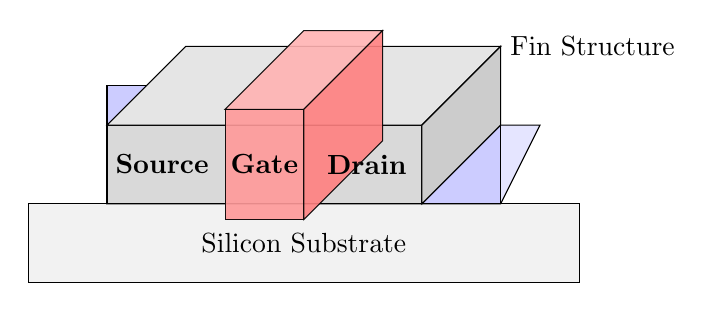
\begin{tikzpicture}
    % Substrate
    \draw[fill=gray!10] (-1,-1) rectangle (6,0);
    \node at (2.5, -0.5) {Silicon Substrate};

    % Fin
    \draw[fill=blue!10] (0,0) -- (5,0) -- (5.5,1) -- (0.5,1) -- cycle; % Top
    \draw[fill=blue!20] (0,0) rectangle (5,1.5); % Front face (actually this is simplified)
    
    % Let's try a better isometric-like view
    % Fin body
    \draw[fill=gray!30] (0,0) -- (4,0) -- (4,1) -- (0,1) -- cycle; % Front
    \draw[fill=gray!20] (0,1) -- (4,1) -- (5,2) -- (1,2) -- cycle; % Top
    \draw[fill=gray!40] (4,0) -- (5,1) -- (5,2) -- (4,1) -- cycle; % Side

    % Gate wrapping around
    \draw[fill=red!40, opacity=0.9] (1.5,-0.2) rectangle (2.5, 1.2); % Front part
    \draw[fill=red!30, opacity=0.9] (1.5,1.2) -- (2.5,1.2) -- (3.5,2.2) -- (2.5,2.2) -- cycle; % Top part
    \draw[fill=red!50, opacity=0.9] (2.5,-0.2) -- (3.5,0.8) -- (3.5,2.2) -- (2.5,1.2) -- cycle; % Side part

    % Labels
    \node at (0.7, 0.5) {\textbf{Source}};
    \node at (3.3, 0.5) {\textbf{Drain}};
    \node at (2, 0.5) {\textbf{Gate}};
    \node[right] at (5,2) {Fin Structure};
\end{tikzpicture}
\caption{FinFET Structure}
\end{figure}

\textbf{Advantages:}

\begin{table}[H]
\centering
\begin{tabulary}{\textwidth}{L L}
\toprule
\textbf{Advantage} & \textbf{Description} \\
\midrule
\textbf{Better Control} & Multiple gates provide superior channel control \\
\textbf{Reduced Leakage} & Lower off-state current due to 3D structure \\
\textbf{Improved Performance} & Higher drive current and faster switching \\
\bottomrule
\end{tabulary}
\caption{FinFET Advantages}
\end{table}

\end{solutionbox}

\begin{mnemonicbox}
\mnemonic{BCR - Better Control Reduces leakage}
\end{mnemonicbox}

\questionmarks{1(b)}{4}{Explain depletion and inversion of MOS structure under external bias}

\begin{solutionbox}
\textbf{Table: MOS Bias Conditions}

\begin{table}[H]
\centering
\begin{tabulary}{\textwidth}{L L L L}
\toprule
\textbf{Bias Type} & \textbf{Gate Voltage} & \textbf{Channel State} & \textbf{Charge Carriers} \\
\midrule
\textbf{Depletion} & Slightly Positive & Depleted & Holes pushed away \\
\textbf{Inversion} & High Positive & Inverted & Electrons attracted \\
\bottomrule
\end{tabulary}
\caption{MOS Bias Conditions}
\end{table}

\begin{figure}[H]
\centering
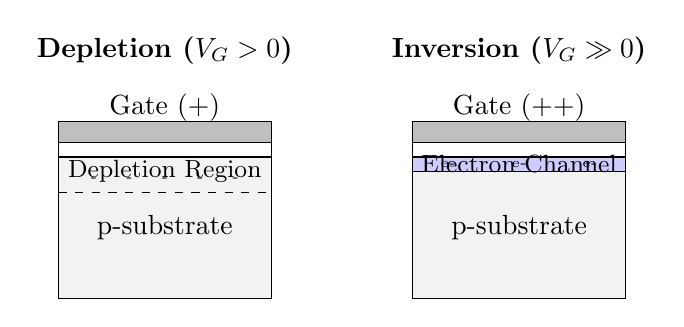
\begin{tikzpicture}[scale=0.9]
    % Depletion Mode
    \begin{scope}
        \node at (1.5, 3.5) {\textbf{Depletion ($V_G > 0$)}};
        \draw[fill=gray!10] (0,0) rectangle (3,2); % Substrate
        \draw[fill=white] (0,2) rectangle (3,2.2); % Oxide
        \draw[fill=gray!50] (0,2.2) rectangle (3,2.5); % Gate
        
        \node at (1.5, 2.7) {Gate (+)};
        \node at (1.5, 1) {p-substrate};
        
        \draw[dashed] (0,1.5) -- (3,1.5);
        \node at (1.5, 1.8) {\small Depletion Region};
        \node[font=\tiny] at (0.5, 1.7) {-}; \node[font=\tiny] at (1.0, 1.7) {-};
        \node[font=\tiny] at (1.5, 1.7) {-}; \node[font=\tiny] at (2.0, 1.7) {-};
        \node[font=\tiny] at (2.5, 1.7) {-};
    \end{scope}

    % Inversion Mode
    \begin{scope}[xshift=5cm]
        \node at (1.5, 3.5) {\textbf{Inversion ($V_G \gg 0$)}};
        \draw[fill=gray!10] (0,0) rectangle (3,2); % Substrate
        \draw[fill=white] (0,2) rectangle (3,2.2); % Oxide
        \draw[fill=gray!50] (0,2.2) rectangle (3,2.5); % Gate
        
        \node at (1.5, 2.7) {Gate (++)};
        \node at (1.5, 1) {p-substrate};
        
        \draw[fill=blue!20] (0,1.8) rectangle (3,2);
        \node at (1.5, 1.9) {\small Electron Channel};
        \node[font=\tiny] at (0.5, 1.9) {e-}; \node[font=\tiny] at (1.5, 1.9) {e-}; \node[font=\tiny] at (2.5, 1.9) {e-};
    \end{scope}
\end{tikzpicture}
\caption{MOS Depletion and Inversion Layers}
\end{figure}

\begin{itemize}
    \item \textbf{Depletion}: Positive gate voltage creates electric field pushing holes away, leaving immobile negative ions.
    \item \textbf{Inversion}: Higher voltage attracts electrons to surface, forming a conducting n-channel.
\end{itemize}

\end{solutionbox}

\begin{mnemonicbox}
\mnemonic{DI - Depletion Inverts to conducting channel}
\end{mnemonicbox}

\questionmarks{1(c)}{7}{Explain n-channel MOSFET with the help of its Current-Voltage characteristics.}

\begin{solutionbox}
\textbf{Table: MOSFET Operating Regions}

\begin{table}[H]
\centering
\begin{tabulary}{\textwidth}{L L L L}
\toprule
\textbf{Region} & \textbf{Condition} & \textbf{Drain Current} & \textbf{Characteristics} \\
\midrule
\textbf{Cut-off} & $V_{GS} < V_{TH}$ & $I_D \approx 0$ & No conduction \\
\textbf{Linear} & $V_{DS} < V_{GS}-V_{TH}$ & $I_D \propto V_{DS}$ & Resistive behavior \\
\textbf{Saturation} & $V_{DS} \geq V_{GS}-V_{TH}$ & $I_D \propto (V_{GS}-V_{TH})^2$ & Current independent of $V_{DS}$ \\
\bottomrule
\end{tabulary}
\caption{MOSFET Operating Regions}
\end{table}

\begin{figure}[H]
\centering
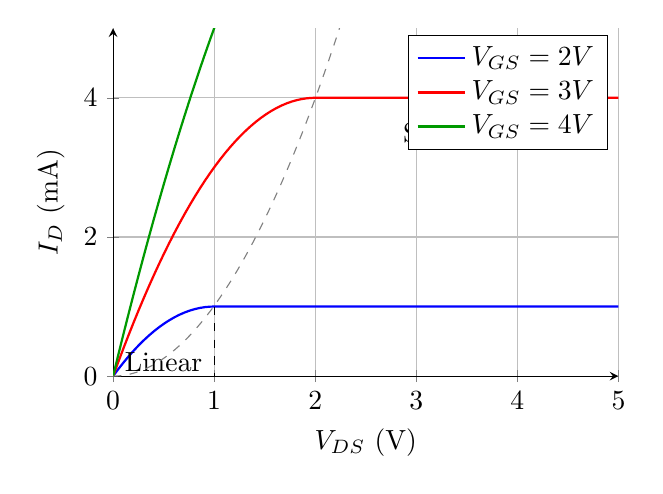
\begin{tikzpicture}
    \begin{axis}[
        width=8cm, height=6cm,
        xlabel={$V_{DS}$ (V)},
        ylabel={$I_D$ (mA)},
        xmin=0, xmax=5,
        ymin=0, ymax=5,
        axis lines=left,
        grid=major
    ]
    \addplot[domain=0:5, samples=100, thick, blue] { (x < 1) ? (2*1*x - x^2) : (1^2) }; 
    \addlegendentry{$V_{GS} = 2V$}
    
    \addplot[domain=0:5, samples=100, thick, red] { (x < 2) ? (2*2*x - x^2) : (2^2) };
    \addlegendentry{$V_{GS} = 3V$}
    
    \addplot[domain=0:5, samples=100, thick, green!60!black] { (x < 3) ? (2*3*x - x^2) : (3^2) };
    \addlegendentry{$V_{GS} = 4V$}
    
    \node at (axis cs: 0.5, 0.2) {Linear};
    \node at (axis cs: 3.5, 3.5) {Saturation};
    \draw[dashed] (axis cs: 1,1) -- (axis cs: 1,0); 
    \draw[dashed, black!50] (axis cs: 0,0) parabola (axis cs:3,9); % Saturation locus
    \end{axis}
\end{tikzpicture}
\caption{MOSFET IV Characteristics}
\end{figure}

\textbf{Key Equations:}
\begin{itemize}
    \item \textbf{Linear}: $I_D = \mu_n C_{ox} \frac{W}{L} [(V_{GS}-V_{TH})V_{DS} - \frac{V_{DS}^2}{2}]$
    \item \textbf{Saturation}: $I_D = \frac{1}{2} \mu_n C_{ox} \frac{W}{L} (V_{GS}-V_{TH})^2$
\end{itemize}

\end{solutionbox}

\begin{mnemonicbox}
\mnemonic{CLS - Cut-off, Linear, Saturation regions}
\end{mnemonicbox}

\questionmarks{1(c OR)}{7}{Define scaling. Compare full voltage scaling with constant voltage scaling. Write the disadvantages of scaling.}

\begin{solutionbox}
\textbf{Definition:} Scaling reduces device dimensions to increase density and performance.

\textbf{Table: Scaling Comparison}

\begin{table}[H]
\centering
\begin{tabulary}{\textwidth}{L L L}
\toprule
\textbf{Parameter} & \textbf{Full Voltage Scaling} & \textbf{Constant Voltage Scaling} \\
\midrule
\textbf{Voltage} & Reduced by $\alpha$ & Remains constant \\
\textbf{Power Density} & Constant & Increases by $\alpha$ \\
\textbf{Electric Field} & Constant & Increases by $\alpha$ \\
\textbf{Performance} & Better & Moderate improvement \\
\bottomrule
\end{tabulary}
\caption{Scaling Comparison}
\end{table}

\textbf{Disadvantages:}
\begin{itemize}
    \item \textbf{Short Channel Effects}: Channel length modulation increases.
    \item \textbf{Hot Carrier Effects}: High electric fields damage devices.
    \item \textbf{Quantum Effects}: Tunneling currents increase significantly.
\end{itemize}

\end{solutionbox}

\begin{mnemonicbox}
\mnemonic{SHQ - Short channel, Hot carriers, Quantum effects}
\end{mnemonicbox}

\questionmarks{2(a)}{3}{Draw two input NAND gate using CMOS.}

\begin{solutionbox}
CMOS NAND gate uses two parallel pMOS transistors and two series nMOS transistors.

\begin{figure}[H]
\centering
\begin{circuitikz}[scale=1.2]
    \draw (0,4) node[vdd] (VDD) {$V_{DD}$};
    \draw (0,4) -- (0,3.5);
    \draw (-1.5,3.5) -- (1.5,3.5); % Top rail
    
    % PMOS Parallel
    \draw (-1.5,3.5) node[pmos, anchor=S] (P1) {};
    \draw (1.5,3.5) node[pmos, anchor=S] (P2) {};
    
    \draw (P1.D) -- (-1.5,1.5) -- (0,1.5);
    \draw (P2.D) -- (1.5,1.5) -- (0,1.5);
    
    % NMOS Series
    \draw (0,1.5) -- (0,1) node[nmos, anchor=D] (N1) {};
    \draw (N1.S) -- (0,-0.5) node[nmos, anchor=D] (N2) {};
    \draw (N2.S) node[ground] {};
    
    % Inputs
    \draw (P1.G) -- ++(-0.5,0) node[left] {A};
    \draw (N1.G) -- ++(-0.5,0) node[left] {A}; % Connect A ideally
    
    \draw (P2.G) -- ++(-0.5,0) node[left] {B};
    \draw (N2.G) -- ++(-0.5,0) node[left] {B}; % Connect B ideally
    
    % Output
    \draw (0,1.5) to[short, -o] (2.5,1.5) node[right] {Y = $\overline{A \cdot B}$};
    
    % Logic connections for correct schematic visualization (schematic line link)
    \draw[dashed] (P1.G) -- (N1.G);
    \draw[dashed] (P2.G) -- (N2.G);
\end{circuitikz}
\caption{2-Input CMOS NAND Gate}
\end{figure}

\textbf{Table: NAND Truth Table}
\begin{table}[H]
\centering
\begin{tabulary}{\textwidth}{C C C}
\toprule
A & B & Y \\
\midrule
0 & 0 & 1 \\
0 & 1 & 1 \\
1 & 0 & 1 \\
1 & 1 & 0 \\
\bottomrule
\end{tabulary}
\caption{NAND Truth Table}
\end{table}

\end{solutionbox}

\begin{mnemonicbox}
\mnemonic{PP-SS: Parallel PMOS, Series NMOS}
\end{mnemonicbox}

\questionmarks{2(b)}{4}{Explain noise immunity and noise margin for nMOS inverter.}

\begin{solutionbox}
\textbf{Table: Noise Parameters}

\begin{table}[H]
\centering
\begin{tabulary}{\textwidth}{L L L}
\toprule
\textbf{Parameter} & \textbf{Definition} & \textbf{Formula} \\
\midrule
\textbf{NMH} & High noise margin & $V_{OH} - V_{IH}$ \\
\textbf{NML} & Low noise margin & $V_{IL} - V_{OL}$ \\
\textbf{Noise Immunity} & Ability to reject noise & Min(NMH, NML) \\
\bottomrule
\end{tabulary}
\caption{Noise Parameters}
\end{table}

\begin{figure}[H]
\centering
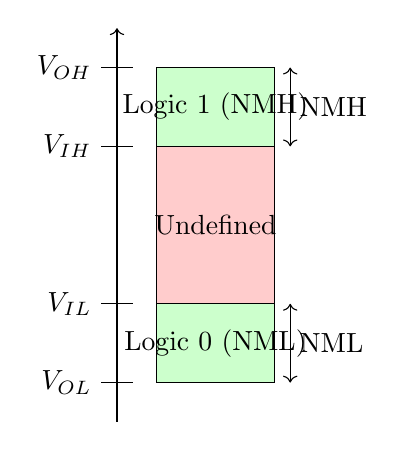
\begin{tikzpicture}
    \draw[->] (0,0) -- (0,5);
    \draw (-0.2, 4.5) node[left] {$V_{OH}$} -- (0.2, 4.5);
    \draw (-0.2, 3.5) node[left] {$V_{IH}$} -- (0.2, 3.5);
    \draw (-0.2, 1.5) node[left] {$V_{IL}$} -- (0.2, 1.5);
    \draw (-0.2, 0.5) node[left] {$V_{OL}$} -- (0.2, 0.5);
    
    \draw[fill=green!20] (0.5, 3.5) rectangle (2, 4.5) node[pos=0.5] {Logic 1 (NMH)};
    \draw[fill=red!20] (0.5, 1.5) rectangle (2, 3.5) node[pos=0.5] {Undefined};
    \draw[fill=green!20] (0.5, 0.5) rectangle (2, 1.5) node[pos=0.5] {Logic 0 (NML)};

    \draw[<->] (2.2, 3.5) -- (2.2, 4.5) node[midway, right] {NMH};
    \draw[<->] (2.2, 0.5) -- (2.2, 1.5) node[midway, right] {NML};
\end{tikzpicture}
\caption{Noise Margins}
\end{figure}

\begin{itemize}
    \item \textbf{$V_{IL}$}: Maximum low input voltage recognized as logic 0.
    \item \textbf{$V_{IH}$}: Minimum high input voltage recognized as logic 1.
    \item \textbf{Good noise immunity}: Large noise margins prevent false switching due to noise.
\end{itemize}

\end{solutionbox}

\begin{mnemonicbox}
\mnemonic{HILOL - High/Low Input/Output Levels}
\end{mnemonicbox}

\questionmarks{2(c)}{7}{Explain Voltage Transfer Characteristics (VTC) of CMOS inverter.}

\begin{solutionbox}
\textbf{Table: VTC Regions}

\begin{table}[H]
\centering
\begin{tabulary}{\textwidth}{C L L L}
\toprule
\textbf{Region} & \textbf{Input Range} & \textbf{Output} & \textbf{Transistor States} \\
\midrule
\textbf{A} & $0$ to $V_{TN}$ & $V_{DD}$ & pMOS ON, nMOS OFF \\
\textbf{B} & $V_{TN}$ to $V_{DD}/2$ & Transition & Both ON (Sat/Lin) \\
\textbf{C} & $V_{DD}/2$ (Threshold) & Rapid Drop & Both Saturation \\
\textbf{D} & $V_{DD}/2$ to $V_{DD}-|V_{TP}|$ & Transition & Both ON (Lin/Sat) \\
\textbf{E} & $V_{DD}-|V_{TP}|$ to $V_{DD}$ & $0V$ & pMOS OFF, nMOS ON \\
\bottomrule
\end{tabulary}
\caption{VTC Regions}
\end{table}

\begin{figure}[H]
\centering
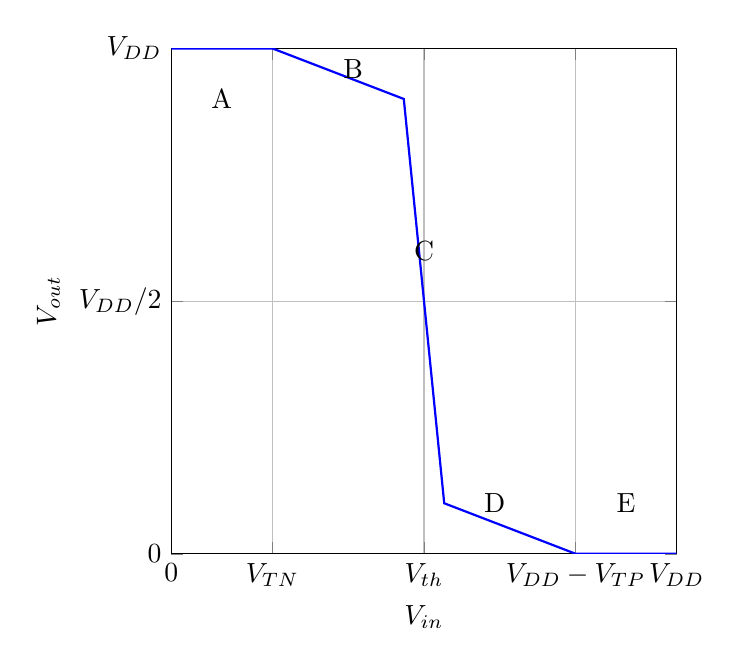
\begin{tikzpicture}
    \begin{axis}[
        width=8cm, height=8cm,
        xlabel={$V_{in}$},
        ylabel={$V_{out}$},
        xmin=0, xmax=5,
        ymin=0, ymax=5,
        grid=major,
        xtick={0,1,2.5,4,5},
        xticklabels={0, $V_{TN}$, $V_{th}$, $V_{DD}-V_{TP}$, $V_{DD}$},
        ytick={0,2.5,5},
        yticklabels={0, $V_{DD}/2$, $V_{DD}$}
    ]
    % Idealized CMOS VTC
    \addplot[thick, blue] coordinates {
        (0,5) (1,5) (2.3, 4.5) (2.5, 2.5) (2.7, 0.5) (4,0) (5,0)
    };
    
    \node at (axis cs: 0.5, 4.5) {A};
    \node at (axis cs: 1.8, 4.8) {B};
    \node at (axis cs: 2.5, 3) {C};
    \node at (axis cs: 3.2, 0.5) {D};
    \node at (axis cs: 4.5, 0.5) {E};
    \end{axis}
\end{tikzpicture}
\caption{CMOS Inverter VTC}
\end{figure}

\textbf{Key Features:}
\begin{itemize}
    \item \textbf{Sharp transition}: Ideal switching behavior at $V_{th}$.
    \item \textbf{High gain}: Large slope in transition region (Region C).
    \item \textbf{Rail-to-rail}: Output swings full supply range ($0$ to $V_{DD}$).
\end{itemize}

\end{solutionbox}

\begin{mnemonicbox}
\mnemonic{ASH - A-region, Sharp transition, High gain}
\end{mnemonicbox}

\questionmarks{2(a OR)}{3}{Implement NOR2 gate using depletion load nMOS.}

\begin{solutionbox}
Depletion load NOR2 uses a depletion nMOS as load and two parallel nMOS as drivers.

\begin{figure}[H]
\centering
\begin{circuitikz}[scale=1.2]
    \draw (0,4) node[vdd] (VDD) {$V_{DD}$};
    \draw (0,4) -- (0,3);
    
    % Depletion Load (nmosD in circuitikz usually, or manual)
    \draw (0,3) node[nmos, anchor=D] (DL) {}; 
    % Circuitikz might not have explicit depletion mode symbol, assume standard with label or modify
    % Actually circuitikz has 'nmosd' for depletion nmos
    
    \draw (DL.S) -- (0,1.5);
    \draw (DL.G) -- ++(-0.5,0) -- (DL.S); % VGS=0 connection
    
    % Parallel nMOS Drivers
    \draw (-1,1.5) -- (0,1.5) -- (1,1.5);
    
    \draw (-1,1.5) -- (-1,1) node[nmos, anchor=D] (N1) {};
    \draw (1,1.5) -- (1,1) node[nmos, anchor=D] (N2) {};
    
    \draw (N1.S) -- (-1,0) -- (0,0);
    \draw (N2.S) -- (1,0) -- (0,0);
    \draw (0,0) node[ground] {};
    
    % Inputs
    \draw (N1.G) -- ++(-0.5,0) node[left] {A};
    \draw (N2.G) -- ++(-0.5,0) node[left] {B};
    
    % Output
    \draw (0,1.5) to[short, -o] (2,1.5) node[right] {Y = $\overline{A+B}$};
    
    \node[right] at (DL.D) {Depletion Load};
\end{circuitikz}
\caption{Depletion Load NOR2}
\end{figure}

\textbf{Table: NOR2 Truth Table}
\begin{table}[H]
\centering
\begin{tabulary}{\textwidth}{C C C}
\toprule
A & B & Y \\
\midrule
0 & 0 & 1 \\
0 & 1 & 0 \\
1 & 0 & 0 \\
1 & 1 & 0 \\
\bottomrule
\end{tabulary}
\caption{NOR2 Truth Table}
\end{table}

\end{solutionbox}

\begin{mnemonicbox}
\mnemonic{DPN - Depletion load, Parallel NMOS}
\end{mnemonicbox}

\questionmarks{2(b OR)}{4}{Differentiate between enhancement load inverter and Depletion load inverter.}

\begin{solutionbox}
\textbf{Table: Load Inverter Comparison}

\begin{table}[H]
\centering
\begin{tabulary}{\textwidth}{L L L}
\toprule
\textbf{Parameter} & \textbf{Enhancement Load} & \textbf{Depletion Load} \\
\midrule
\textbf{Threshold Voltage} & $V_T > 0$ & $V_T < 0$ \\
\textbf{Gate Connection} & $V_{GS} = V_{DS}$ & $V_{GS} = 0$ \\
\textbf{Logic High ($V_{OH}$)} & $V_{DD} - V_T$ & $V_{DD}$ \\
\textbf{Power Consumption} & Higher & Lower \\
\textbf{Switching Speed} & Slower & Faster \\
\bottomrule
\end{tabulary}
\caption{Inverter Load Types Comparison}
\end{table}

\end{solutionbox}

\begin{mnemonicbox}
\mnemonic{EPDLH - Enhancement Positive, Depletion Lower power, Higher speed}
\end{mnemonicbox}

\questionmarks{2(c OR)}{7}{Explain Depletion load nMOS inverter with its VTC.}

\begin{solutionbox}
\textbf{Circuit Operation:}
\begin{itemize}
    \item \textbf{Load transistor}: Always conducting ($V_{GS} = 0, V_T < 0$). Acts as a constant current source.
    \item \textbf{Driver transistor}: Controlled by input voltage ($V_{in}$).
    \item \textbf{Output}: Determined by voltage divider action between load and driver resistances.
\end{itemize}

\begin{figure}[H]
\centering
\begin{circuitikz}[scale=1]
    \draw (0,4) node[vdd] (VDD) {$V_{DD}$};
    \draw (0,4) -- (0,3) node[nmos, anchor=D] (L) {}; % Depletion load
    \draw (L.S) -- (0,1.5);
    \draw (L.G) -- ++(-0.5,0) -- (L.S);
    
    \draw (0,1.5) -- (0,1) node[nmos, anchor=D] (D) {}; % Enh Driver
    \draw (D.S) node[ground] {};
    
    \draw (D.G) -- ++(-0.5,0) node[left] {$V_{in}$};
    \draw (0,1.5) to[short, -o] (1.5,1.5) node[right] {$V_{out}$};
    
    \node[right] at (L.D) {Depletion Load};
    \node[right] at (D.D) {Driver};
\end{circuitikz}
\caption{Depletion Load Inverter}
\end{figure}

\textbf{Table: Operating Points}
\begin{table}[H]
\centering
\begin{tabulary}{\textwidth}{L L L L}
\toprule
\textbf{Input State} & \textbf{Driver} & \textbf{Load} & \textbf{Output} \\
\midrule
$\mathbf{V_{in} = 0}$ & OFF & ON (Linear) & $V_{DD}$ \\
$\mathbf{V_{in} = V_{DD}}$ & ON (Linear) & ON (Sat) & $\approx 0V$ \\
\bottomrule
\end{tabulary}
\caption{Inverter Operating Points}
\end{table}

\textbf{VTC Characteristics:}
\begin{itemize}
    \item \textbf{$V_{OH}$}: Reaches full $V_{DD}$ (unlike enhancement load which drops $V_T$).
    \item \textbf{$V_{OL}$}: Low voltage close to 0V.
    \item \textbf{Transition}: Sharp switching due to better load characteristics.
\end{itemize}

\end{solutionbox}

\begin{mnemonicbox}
\mnemonic{DLB - Depletion Load gives Better high output}
\end{mnemonicbox}

\questionmarks{3(a)}{3}{Implement EX-OR using Depletion load nMOS.}

\begin{solutionbox}
To implement XOR ($Y = A \oplus B = A\bar{B} + \bar{A}B$) using depletion load nMOS logic (which implements $\overline{\text{Pull-Down}}$), we organize the pull-down network to realize the complement of XOR, which is XNOR ($AB + \bar{A}\bar{B}$).
A standard implementation uses 4 transistors in the pull-down network to realize $Y = \overline{(A+\bar{B})(\bar{A}+B)} = A \oplus B$.

\begin{figure}[H]
\centering
\begin{circuitikz}[scale=1]
    \draw (0,5) node[vdd] (VDD) {$V_{DD}$};
    \draw (0,5) -- (0,4) node[nmos, anchor=D] (L) {}; % Depletion Load
    \draw (L.S) -- (0,3);
    \draw (L.G) -- ++(-0.5,0) -- (L.S);
    
    % Pull Down Network implementing (A + B')(A' + B)
    % Series of two parallel blocks
    \draw (0,3) -- (0,2.5);
    
    % Block 1: A || B'
    \draw (0,2.5) -- (-1.5,2.5) -- (-1.5,1.5) node[nmos, anchor=D] (NA) {};
    \draw (0,2.5) -- (1.5,2.5) -- (1.5,1.5) node[nmos, anchor=D] (NBp) {};
    
    \draw (NA.S) -- (-1.5,0.5);
    \draw (NBp.S) -- (1.5,0.5);
    
    % Connect Block 1 to Block 2
    \draw (-1.5,0.5) -- (0,0.5) -- (1.5,0.5);
    
    % Block 2: A' || B
    \draw (0,0.5) -- (-1.5,0.5) -- (-1.5,-0.5) node[nmos, anchor=D] (NAp) {};
    \draw (0,0.5) -- (1.5,0.5) -- (1.5,-0.5) node[nmos, anchor=D] (NB) {};
    
    \draw (NAp.S) -- (-1.5,-1.5) -- (0,-1.5);
    \draw (NB.S) -- (1.5,-1.5) -- (0,-1.5);
    \draw (0,-1.5) node[ground] {};
    
    % Inputs
    \draw (NA.G) -- ++(-0.2,0) node[left] {A};
    \draw (NBp.G) -- ++(-0.2,0) node[left] {$B'$};
    \draw (NAp.G) -- ++(-0.2,0) node[left] {$A'$};
    \draw (NB.G) -- ++(-0.2,0) node[left] {B};
    
    % Output
    \draw (0,3) to[short, -o] (2.5,3) node[right] {$Y = A \oplus B$};
    
    \node[right] at (L.D) {Depletion Load};
\end{circuitikz}
\caption{Depletion Load NMOS EX-OR Gate}
\end{figure}

\textbf{Logic Equation:}
$Y = \overline{(A + \bar{B}) \cdot (\bar{A} + B)} = \overline{A\bar{A} + AB + \bar{B}\bar{A} + \bar{B}B} = \overline{0 + AB + \bar{A}\bar{B} + 0} = \overline{A \odot B} = A \oplus B$

\end{solutionbox}

\begin{mnemonicbox}
\mnemonic{XOR - eXclusive OR, different inputs give 1}
\end{mnemonicbox}

\questionmarks{3(b)}{4}{Explain design hierarchy with example.}

\begin{solutionbox}
\textbf{Table: Hierarchy Levels}

\begin{table}[H]
\centering
\begin{tabulary}{\textwidth}{L L L}
\toprule
\textbf{Level} & \textbf{Component} & \textbf{Example} \\
\midrule
\textbf{System} & Complete chip & Microprocessor \\
\textbf{Module} & Functional blocks & ALU, Memory \\
\textbf{Gate} & Logic gates & NAND, NOR \\
\textbf{Transistor} & Individual devices & MOSFET \\
\bottomrule
\end{tabulary}
\caption{Design Hierarchy Levels}
\end{table}

\begin{figure}[H]
\centering
\begin{tikzpicture}[gtu tree]
    \node [gtu root] {System Level (CPU)}
        child { node [gtu child] {Module Level (ALU)}
            child { node [gtu block] {Gate Level (Adder)}
                child { node [gtu block, fill=orange!10] {Transistor Level (MOSFET)} }
            }
        }
        child { node [gtu child] {Module Level (Registers)} };
\end{tikzpicture}
\caption{Design Hierarchy Tree}
\end{figure}

\textbf{Benefits:}
\begin{itemize}
    \item \textbf{Modularity}: Independent design and testing of blocks.
    \item \textbf{Reusability}: Common blocks (like adders) used multiple times.
    \item \textbf{Maintainability}: Easy debugging and modification.
\end{itemize}

\end{solutionbox}

\begin{mnemonicbox}
\mnemonic{SMG-T: System, Module, Gate, Transistor levels}
\end{mnemonicbox}

\questionmarks{3(c)}{7}{Draw and explain Y chart design flow.}

\begin{solutionbox}
The Y-chart represents the three domains of VLSI design: Behavioral, Structural, and Physical.

\begin{figure}[H]
\centering
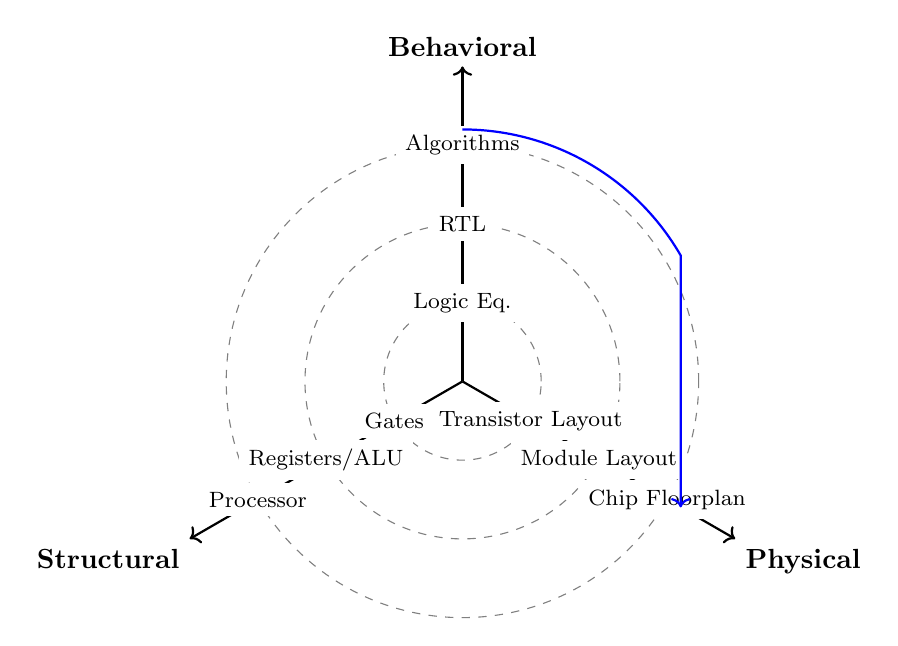
\begin{tikzpicture}
    % Axes
    \draw[thick, ->] (0,0) -- (90:4) node[above] {\textbf{Behavioral}};
    \draw[thick, ->] (0,0) -- (210:4) node[below left] {\textbf{Structural}};
    \draw[thick, ->] (0,0) -- (330:4) node[below right] {\textbf{Physical}};
    
    % Concentric circles for levels
    \foreach \r in {1,2,3} {
        \draw[dashed, gray] (0,0) circle (\r);
    }
    
    % Items
    \node[font=\footnotesize, fill=white] at (90:3) {Algorithms};
    \node[font=\footnotesize, fill=white] at (90:2) {RTL};
    \node[font=\footnotesize, fill=white] at (90:1) {Logic Eq.};
    
    \node[font=\footnotesize, fill=white] at (210:3) {Processor};
    \node[font=\footnotesize, fill=white] at (210:2) {Registers/ALU};
    \node[font=\footnotesize, fill=white] at (210:1) {Gates};
    
    \node[font=\footnotesize, fill=white] at (330:3) {Chip Floorplan};
    \node[font=\footnotesize, fill=white] at (330:2) {Module Layout};
    \node[font=\footnotesize, fill=white] at (330:1) {Transistor Layout};
    
    % Spiral flow
    \draw[->, blue, thick] (90:3.2) arc (90:30:3.2) -- (330:3.2);
\end{tikzpicture}
\caption{Gajski-Kuhn Y-Chart}
\end{figure}

\textbf{Table: Y-Chart Domains}
\begin{table}[H]
\centering
\begin{tabulary}{\textwidth}{L L L}
\toprule
\textbf{Domain} & \textbf{Description} & \textbf{Examples} \\
\midrule
\textbf{Behavioral} & What system does & Algorithms, RTL \\
\textbf{Structural} & How it's organized & Architecture, Gates \\
\textbf{Physical} & Where components placed & Floorplan, Layout \\
\bottomrule
\end{tabulary}
\caption{Y-Chart Domains}
\end{table}

\textbf{Design Flow:}
\begin{itemize}
    \item \textbf{Top-down}: Behavioral $\to$ Structural $\to$ Physical.
    \item \textbf{Bottom-up}: Physical constraints influence upper levels.
\end{itemize}

\end{solutionbox}

\begin{mnemonicbox}
\mnemonic{BSP - Behavioral, Structural, Physical domains}
\end{mnemonicbox}

\questionmarks{3(a OR)}{3}{Implement NAND2 - SR latch using CMOS}

\begin{solutionbox}
NAND SR Latch consists of two cross-coupled NAND gates.

\begin{figure}[H]
\centering
\begin{circuitikz}
    \draw (0,0) node[nand port] (N1) {};
    \draw (0,-2) node[nand port] (N2) {};
    
    % Inputs
    \draw (N1.in 1) -- ++(-1,0) node[left] {$\bar{S}$};
    \draw (N2.in 2) -- ++(-1,0) node[left] {$\bar{R}$};
    
    % Outputs
    \draw (N1.out) -- ++(1,0) node[right] {$Q$};
    \draw (N2.out) -- ++(1,0) node[right] {$\bar{Q}$};
    
    % Cross coupling
    \draw (N1.in 2) -- ++(-0.5,0) -- ++(0,-0.5) -- ++(2.5,-1.2) -- (N2.out);
    \draw (N2.in 1) -- ++(-0.5,0) -- ++(0,0.5) -- ++(2.5,1.2) -- (N1.out);
\end{circuitikz}
\caption{CMOS NAND SR Latch}
\end{figure}

\textbf{Table: SR Latch Operation}
\begin{table}[H]
\centering
\begin{tabulary}{\textwidth}{C C C C L}
\toprule
S & R & Q & Q' & State \\
\midrule
0 & 0 & 1 & 1 & Invalid \\
0 & 1 & 1 & 0 & Set \\
1 & 0 & 0 & 1 & Reset \\
1 & 1 & Q & Q' & Hold \\
\bottomrule
\end{tabulary}
\caption{NAND SR Latch Truth Table (Active Low Inputs)}
\end{table}

\end{solutionbox}

\begin{mnemonicbox}
\mnemonic{SR-HRI: Set, Reset, Hold, Invalid states}
\end{mnemonicbox}

\questionmarks{3(b OR)}{4}{Which method is used to transfer pattern or mask on the silicon wafer? Explain it with neat diagrams}

\begin{solutionbox}
\textbf{Method}: \textbf{Photolithography} is used to transfer geometric shapes on a mask to the surface of a silicon wafer.

\begin{figure}[H]
\centering
\begin{tikzpicture}[node distance=1.5cm]
    \node [gtu process] (coat) {1. Coating\\(Apply Photoresist)};
    \node [gtu process, right=of coat] (expose) {2. Exposure\\(UV Light via Mask)};
    \node [gtu process, right=of expose] (develop) {3. Development\\(Remove Exposed)};
    
    \draw [gtu arrow] (coat) -- (expose);
    \draw [gtu arrow] (expose) -- (develop);
    
    % Simplified diagrams below nodes
    \draw[fill=gray!20] (-1,-1) rectangle (1,-1.5); % Wafer
    \draw[fill=red!20] (-1,-1) rectangle (1,-0.8); % Resist
    \node[below=2cm of coat] {PR Coated Wafer};
    
    \draw[fill=gray!20] (3.5,-1) rectangle (5.5,-1.5);
    \draw[fill=red!20] (3.5,-1) rectangle (5.5,-0.8);
    \draw[thick] (4,-0.3) -- (5,-0.3); % Mask
    \draw[->, yellow!80!black] (4.5, 0.2) -- (4.5, -0.3); % UV
    \node[below=2cm of expose] {UV Exposure};
    
    \draw[fill=gray!20] (8,-1) rectangle (10,-1.5);
    \draw[fill=red!20] (8,-1) rectangle (8.5,-0.8); 
    \draw[fill=red!20] (9.5,-1) rectangle (10,-0.8); % Patterned
    \node[below=2cm of develop] {Pattern Defined};
\end{tikzpicture}
\caption{Photolithography Process}
\end{figure}

\textbf{Process Steps:}
\begin{itemize}
    \item \textbf{Coating}: Applying a thin layer of photoresist.
    \item \textbf{Exposure}: Exposing resist to UV light through a mask.
    \item \textbf{Development}: Dissolving the exposed (positive) or unexposed (negative) resist.
\end{itemize}

\end{solutionbox}

\begin{mnemonicbox}
\mnemonic{CED - Coating, Exposure, Development}
\end{mnemonicbox}

\questionmarks{3(c OR)}{7}{Which are the methods used to deposit metal in MOSFET fabrication? Explain deposition in detail with proper diagram.}

\begin{solutionbox}
\textbf{Table: Metal Deposition Methods}

\begin{table}[H]
\centering
\begin{tabulary}{\textwidth}{L L L}
\toprule
\textbf{Method} & \textbf{Technique} & \textbf{Application} \\
\midrule
\textbf{PVD} & Sputtering, Evaporation & Aluminum, Copper \\
\textbf{CVD} & CVD, PECVD & Tungsten, Titanium \\
\textbf{Electroplating} & Electrochemical & Copper interconnects \\
\bottomrule
\end{tabulary}
\caption{Metal Deposition Methods}
\end{table}

\textbf{Sputtering Process:}
In sputtering, ions from a plasma are accelerated towards a target material, ejecting atoms which settle on the wafer.

\begin{figure}[H]
\centering
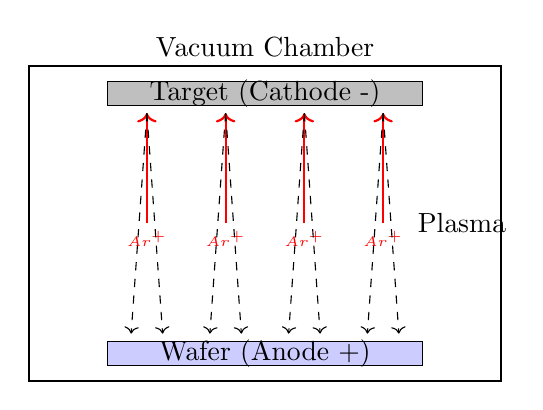
\begin{tikzpicture}
    % Chamber
    \draw[thick] (0,0) rectangle (6,4);
    \node[above] at (3,4) {Vacuum Chamber};
    
    % Target
    \draw[fill=gray!50] (1,3.5) rectangle (5,3.8);
    \node at (3,3.65) {Target (Cathode -)};
    
    % Wafer
    \draw[fill=blue!20] (1,0.2) rectangle (5,0.5);
    \node at (3,0.35) {Wafer (Anode +)};
    
    % Ions
    \foreach \x in {1.5, 2.5, 3.5, 4.5} {
        \draw[->, red, thick] (\x, 2) -- (\x, 3.4); % Ions hitting target
        \node[red, font=\tiny] at (\x, 1.8) {$Ar^+$};
        
        \draw[->, black, dashed] (\x, 3.4) -- (\x-0.2, 0.6); % Atoms falling
        \draw[->, black, dashed] (\x, 3.4) -- (\x+0.2, 0.6);
    }
    \node at (5.5, 2) {Plasma};
\end{tikzpicture}
\caption{Sputtering System}
\end{figure}

\textbf{Advantages:}
\begin{itemize}
    \item \textbf{Uniform thickness}: Excellent step coverage.
    \item \textbf{Low temperature}: Preserves device integrity.
    \item \textbf{Variety}: Can deposit alloys and compounds.
\end{itemize}

\end{solutionbox}

\begin{mnemonicbox}
\mnemonic{IBE-DC: Ion Bombardment Ejects atoms for Deposition Control}
\end{mnemonicbox}

\questionmarks{4(a)}{3}{Implement Z= ((A+B+C)·(D+E+F). G)' with depletion nMOS load.}

\begin{solutionbox}
The logic function $Z = \overline{(A+B+C) \cdot (D+E+F) \cdot G}$ is implemented using a depletion load and a pull-down network. The pull-down network consists of three series blocks corresponding to the AND operations:
1. Parallel inputs A, B, C (OR)
2. Parallel inputs D, E, F (OR)
3. Single input G
Since these are ANDed, the blocks are in series.

\begin{figure}[H]
\centering
\begin{circuitikz}[scale=1]
    \draw (0,6) node[vdd] (VDD) {$V_{DD}$};
    \draw (0,6) -- (0,5) node[nmos, anchor=D] (L) {}; % Depletion Load
    \draw (L.S) -- (0,4.5);
    \draw (L.G) -- ++(-0.5,0) -- (L.S);
    
    % Output Z
    \draw (0,4.5) to[short, -o] (3,4.5) node[right] {$Z$};
    
    % Pull Down Network
    % Series layout
    
    % Block 1: Parallel A, B, C
    \draw (0,4.5) -- (0,4);
    \draw (0,4) -- (-2,4) -- (-2,3) node[nmos, anchor=D] (NA) {};
    \draw (0,4) -- (0,3) node[nmos, anchor=D] (NB) {};
    \draw (0,4) -- (2,4) -- (2,3) node[nmos, anchor=D] (NC) {};
    
    \draw (NA.S) -- (-2,2);
    \draw (NB.S) -- (0,2);
    \draw (NC.S) -- (2,2);
    \draw (-2,2) -- (2,2); % Combine sources
    
    % Block 2: Parallel D, E, F
    \draw (0,2) -- (0,1.5);
    \draw (0,1.5) -- (-2,1.5) -- (-2,0.5) node[nmos, anchor=D] (ND) {};
    \draw (0,1.5) -- (0,0.5) node[nmos, anchor=D] (NE) {};
    \draw (0,1.5) -- (2,1.5) -- (2,0.5) node[nmos, anchor=D] (NF) {};
    
    \draw (ND.S) -- (-2,-0.5);
    \draw (NE.S) -- (0,-0.5);
    \draw (NF.S) -- (2,-0.5);
    \draw (-2,-0.5) -- (2,-0.5); % Combine sources
    
    % Block 3: Series G (Single)
    \draw (0,-0.5) -- (0,-1) node[nmos, anchor=D] (NG) {};
    \draw (NG.S) node[ground] {};
    
    % Inputs
    \draw (NA.G) -- ++(-0.2,0) node[left] {A};
    \draw (NB.G) -- ++(-0.2,0) node[left] {B};
    \draw (NC.G) -- ++(-0.2,0) node[left] {C};
    
    \draw (ND.G) -- ++(-0.2,0) node[left] {D};
    \draw (NE.G) -- ++(-0.2,0) node[left] {E};
    \draw (NF.G) -- ++(-0.2,0) node[left] {F};
    
    \draw (NG.G) -- ++(-0.2,0) node[left] {G};
    
    \node[right] at (L.D) {Depletion Load};
\end{circuitikz}
\caption{Logic Implementation of Z}
\end{figure}

\end{solutionbox}

\begin{mnemonicbox}
\mnemonic{POI - Parallel OR, Inversion at output}
\end{mnemonicbox}

\questionmarks{4(b)}{4}{List and explain the design styles used in VERILOG.}

\begin{solutionbox}
\textbf{Table: Verilog Design Styles}

\begin{table}[H]
\centering
\begin{tabulary}{\textwidth}{L L L L}
\toprule
\textbf{Style} & \textbf{Description} & \textbf{Use Case} & \textbf{Example} \\
\midrule
\textbf{Behavioral} & Algorithm description & High-level modeling & \code{always} blocks \\
\textbf{Dataflow} & Boolean expressions & Combinational logic & \code{assign} statements \\
\textbf{Structural} & Component instantiation & Hierarchical design & module connections \\
\textbf{Gate-level} & Primitive gates & Low-level design & \code{and}, \code{or}, \code{not} gates \\
\bottomrule
\end{tabulary}
\caption{Verilog Design Styles}
\end{table}

\textbf{Characteristics:}
\begin{itemize}
    \item \textbf{Behavioral}: Describes what circuit does (functionality).
    \item \textbf{Structural}: Shows how components connect (netlist).
    \item \textbf{Mixed}: Combines multiple styles for complex ideas.
\end{itemize}

\end{solutionbox}

\begin{mnemonicbox}
\mnemonic{BDSG - Behavioral, Dataflow, Structural, Gate-level}
\end{mnemonicbox}

\questionmarks{4(c)}{7}{Implement NAND2 SR latch using CMOS and also implement NOR2 SR latch using CMOS.}

\begin{solutionbox}
\textbf{NAND2 SR Latch (Verilog):}
\begin{lstlisting}[language=Verilog]
module nand_sr_latch(
    input S, R,
    output Q, Q_bar
);
    nand(Q, S, Q_bar);
    nand(Q_bar, R, Q);
endmodule
\end{lstlisting}

\textbf{NOR2 SR Latch (Verilog):}
\begin{lstlisting}[language=Verilog]
module nor_sr_latch(
    input S, R,
    output Q, Q_bar
);
    nor(Q_bar, R, Q);
    nor(Q, S, Q_bar);
endmodule
\end{lstlisting}

\textbf{Comparison:}
\begin{itemize}
    \item \textbf{NAND}: Set/Reset with low inputs (Active Low).
    \item \textbf{NOR}: Set/Reset with high inputs (Active High).
\end{itemize}

\end{solutionbox}

\begin{mnemonicbox}
\mnemonic{NAND-Low, NOR-High active}
\end{mnemonicbox}

\questionmarks{4(a OR)}{3}{Implement Y= (ABC + DE + F)' with depletion nMOS load.}

\begin{solutionbox}
The logic function $Y = \overline{(ABC) + (DE) + F}$ implements Sum of Products (ORing of AND terms).
The pull-down network consists of three parallel branches:
1. A, B, C in Series (AND)
2. D, E in Series (AND)
3. F Single

\begin{figure}[H]
\centering
\begin{circuitikz}[scale=1]
    \draw (0,5) node[vdd] (VDD) {$V_{DD}$};
    \draw (0,5) -- (0,4) node[nmos, anchor=D] (L) {}; % Depletion Load
    \draw (L.S) -- (0,3.5);
    \draw (L.G) -- ++(-0.5,0) -- (L.S);
    
    % Output Y
    \draw (0,3.5) to[short, -o] (3,3.5) node[right] {$Y$};
    
    % Pull Down Network
    % Parallel layout
    
    \draw (0,3.5) -- (0,3);
    
    % Branch 1: ABC Series (-2 x)
    \draw (0,3) -- (-2,3) -- (-2,2.5) node[nmos, anchor=D] (NA) {};
    \draw (NA.S) -- (-2,1.5) node[nmos, anchor=D] (NB) {};
    \draw (NB.S) -- (-2,0.5) node[nmos, anchor=D] (NC) {};
    \draw (NC.S) -- (-2,-0.5) node[ground] {};
    
    % Branch 2: DE Series (0 x)
    \draw (0,3) -- (0,2) node[nmos, anchor=D] (ND) {};
    \draw (ND.S) -- (0,1) node[nmos, anchor=D] (NE) {};
    \draw (NE.S) -- (0,-0.5) node[ground] {};
    
    % Branch 3: F Single (2 x)
    \draw (0,3) -- (2,3) -- (2,1.5) node[nmos, anchor=D] (NF) {};
    \draw (NF.S) -- (2,-0.5) node[ground] {};
    
    % Inputs
    \draw (NA.G) -- ++(-0.2,0) node[left] {A};
    \draw (NB.G) -- ++(-0.2,0) node[left] {B};
    \draw (NC.G) -- ++(-0.2,0) node[left] {C};
    
    \draw (ND.G) -- ++(-0.2,0) node[left] {D};
    \draw (NE.G) -- ++(-0.2,0) node[left] {E};
    
    \draw (NF.G) -- ++(-0.2,0) node[left] {F};
    
\end{circuitikz}
\caption{Logic Implementation of Y}
\end{figure}

\end{solutionbox}

\begin{mnemonicbox}
\mnemonic{SSS-I: Series-Series-Single with Inversion}
\end{mnemonicbox}

\questionmarks{4(b OR)}{4}{Write Verilog Code to implement full adder.}

\begin{solutionbox}
\begin{lstlisting}[language=Verilog]
module full_adder(
    input a, b, cin,
    output sum, cout
);
    assign sum = a ^ b ^ cin;
    assign cout = (a & b) | (cin & (a ^ b));
endmodule
\end{lstlisting}

\textbf{Logic Functions:}
\begin{itemize}
    \item \textbf{Sum}: Triple XOR operation ($A \oplus B \oplus C_{in}$)
    \item \textbf{Carry}: Majority function of inputs ($AB + B C_{in} + A C_{in}$)
\end{itemize}

\end{solutionbox}

\begin{mnemonicbox}
\mnemonic{XOR-Sum, Majority-Carry}
\end{mnemonicbox}

\questionmarks{4(c OR)}{7}{Implement Y =(S1'S0'I0 + S1'S0 I1 + S1 S0' I2 + S1 S2 I3) using depletion load}

\begin{solutionbox}
\textbf{4:1 Multiplexer Verilog Code} (Assuming S2 corresponds to S0 in context of 4-input):

\begin{lstlisting}[language=Verilog]
// 4:1 Multiplexer implementation
module mux_4to1(
    input [1:0] sel,  // S1, S0
    input [3:0] data, // I3, I2, I1, I0
    output Y
);
    assign Y = (sel == 2'b00) ? data[0] :
               (sel == 2'b01) ? data[1] :
               (sel == 2'b10) ? data[2] :
                                data[3];
endmodule
\end{lstlisting}

\textbf{Table: Multiplexer Selection}

\begin{table}[H]
\centering
\begin{tabulary}{\textwidth}{C C C L}
\toprule
S1 & S0 & Selected Input & Output \\
\midrule
0 & 0 & I0 & $Y = I0$ \\
0 & 1 & I1 & $Y = I1$ \\
1 & 0 & I2 & $Y = I2$ \\
1 & 1 & I3 & $Y = I3$ \\
\bottomrule
\end{tabulary}
\caption{Multiplexer Selection}
\end{table}

\end{solutionbox}

\begin{mnemonicbox}
\mnemonic{DAO - Decoder, AND gates, OR combination}
\end{mnemonicbox}

\questionmarks{5(a)}{3}{Implement the logic function G = (PQR +U(S+T))' using CMOS}

\begin{solutionbox}
The function $G = \overline{(PQR) + U(S+T)}$ requires a CMOS implementation.
\textbf{Pull-Down Network (PDN)}: Implements $(PQR) + U(S+T)$ via nMOS.
\begin{itemize}
    \item $P, Q, R$ in Series (AND).
    \item $S, T$ in Parallel (OR) is correct for $(S+T)$.
    \item $U$ in Series with $(S || T)$.
    \item The block $(P-Q-R)$ is in Parallel with $(U-(S||T))$.
\end{itemize}

\textbf{Pull-Up Network (PUN)}: Implements dual via pMOS.
\begin{itemize}
    \item $P, Q, R$ in Parallel.
    \item $S, T$ in Series.
    \item $U$ in Parallel with $(S-T)$.
    \item The block $(P||Q||R)$ is in Series with $(U || (S-T))$.
\end{itemize}

\begin{figure}[H]
\centering
\begin{circuitikz}[scale=0.9]
    \draw (0,8) node[vdd] (VDD) {$V_{DD}$};
    
    % PUN
    % Top Block: P || Q || R
    \draw (0,8) -- (0,7.5);
    \draw (0,7.5) -- (-2,7.5) -- (-2,6.5) node[pmos, anchor=S] (P) {};
    \draw (0,7.5) -- (0,6.5) node[pmos, anchor=S] (Q) {};
    \draw (0,7.5) -- (2,7.5) -- (2,6.5) node[pmos, anchor=S] (R) {};
    
    \draw (P.D) -- (-2,5.5);
    \draw (Q.D) -- (0,5.5);
    \draw (R.D) -- (2,5.5);
    \draw (-2,5.5) -- (2,5.5); % Merge points
    
    % Connect Top to Bottom PUN
    \draw (0,5.5) -- (0,5);
    
    % Bottom Block: U || (S-T)
    \draw (0,5) -- (-2,5) -- (-2,4) node[pmos, anchor=S] (U) {};
    \draw (0,5) -- (2,5) -- (2,4) node[pmos, anchor=S] (S) {};
    
    \draw (S.D) -- (2,3.5) node[pmos, anchor=S] (T) {};
    
    \draw (U.D) -- (-2,2.5);
    \draw (T.D) -- (2,2.5);
    \draw (-2,2.5) -- (2,2.5); % Output node Y
    
    \draw (0,2.5) to[short, -o] (4,2.5) node[right] {$G$};
    
    % PDN
    % Parallel Branches
    \draw (0,2.5) -- (0,2);
    
    % Branch 1: P-Q-R Series
    \draw (0,2) -- (-3,2) -- (-3,1.5) node[nmos, anchor=D] (nP) {};
    \draw (nP.S) -- (-3,0.5) node[nmos, anchor=D] (nQ) {};
    \draw (nQ.S) -- (-3,-0.5) node[nmos, anchor=D] (nR) {};
    \draw (nR.S) -- (-3,-1.5);
    
    % Branch 2: U Series (S || T)
    \draw (0,2) -- (3,2) -- (3,1.5) node[nmos, anchor=D] (nU) {};
    \draw (nU.S) -- (3,0.5);
    
    \draw (3,0.5) -- (1.5,0.5) -- (1.5,-0.5) node[nmos, anchor=D] (nS) {};
    \draw (3,0.5) -- (4.5,0.5) -- (4.5,-0.5) node[nmos, anchor=D] (nT) {};
    
    \draw (nS.S) -- (1.5,-1.5) -- (3,-1.5);
    \draw (nT.S) -- (4.5,-1.5) -- (3,-1.5);
    
    \draw (3,-1.5) -- (-3,-1.5); % Common Ground
    \draw (0,-1.5) node[ground] {};
    
    % Labels
    \draw (P.G) node[left] {P}; \draw (nP.G) node[left] {P};
    \draw (Q.G) node[left] {Q}; \draw (nQ.G) node[left] {Q};
    \draw (R.G) node[left] {R}; \draw (nR.G) node[left] {R};
    \draw (U.G) node[left] {U}; \draw (nU.G) node[left] {U};
    \draw (S.G) node[left] {S}; \draw (nS.G) node[left] {S};
    \draw (T.G) node[left] {T}; \draw (nT.G) node[left] {T};
    
\end{circuitikz}
\caption{CMOS Implementation of Logic G}
\end{figure}

\end{solutionbox}

\begin{mnemonicbox}
\mnemonic{PSSP - Parallel Series Series Parallel}
\end{mnemonicbox}

\questionmarks{5(b)}{4}{Implement 8x1 multiplexer using Verilog}

\begin{solutionbox}
\begin{lstlisting}[language=Verilog]
module mux_8to1(
    input [2:0] sel,     // 3-bit select
    input [7:0] data,    // 8 data inputs
    output reg Y         // Output
);
    always @(*) begin
        case(sel)
            3'b000: Y = data[0];
            3'b001: Y = data[1];
            3'b010: Y = data[2];
            3'b011: Y = data[3];
            3'b100: Y = data[4];
            3'b101: Y = data[5];
            3'b110: Y = data[6];
            3'b111: Y = data[7];
        endcase
    end
endmodule
\end{lstlisting}

\textbf{Table: 8:1 MUX Selection}
\begin{table}[H]
\centering
\begin{tabulary}{\textwidth}{C C C L}
\toprule
S2 & S1 & S0 & Output \\
\midrule
0 & 0 & 0 & data[0] \\
0 & 0 & 1 & data[1] \\
1 & 0 & 0 & data[4] \\
1 & 1 & 1 & data[7] \\
\bottomrule
\end{tabulary}
\caption{8:1 MUX Truth Table (Partial)}
\end{table}

\end{solutionbox}

\begin{mnemonicbox}
\mnemonic{Case-Always: Use case statement in always block}
\end{mnemonicbox}

\questionmarks{5(c)}{7}{Implement 4 bit full adder using structural modeling style in Verilog.}

\begin{solutionbox}
\textbf{Verilog Code (Structural):}

\begin{lstlisting}[language=Verilog]
module full_adder(
    input a, b, cin,
    output sum, cout
);
    assign sum = a ^ b ^ cin;
    assign cout = (a & b) | (cin & (a ^ b));
endmodule

module full_adder_4bit(
    input [3:0] a, b,
    input cin,
    output [3:0] sum,
    output cout
);
    wire c1, c2, c3;
    
    // Instantiating 4 Full Adders
    full_adder fa0(.a(a[0]), .b(b[0]), .cin(cin), 
                   .sum(sum[0]), .cout(c1));
    full_adder fa1(.a(a[1]), .b(b[1]), .cin(c1), 
                   .sum(sum[1]), .cout(c2));
    full_adder fa2(.a(a[2]), .b(b[2]), .cin(c2), 
                   .sum(sum[2]), .cout(c3));
    full_adder fa3(.a(a[3]), .b(b[3]), .cin(c3), 
                   .sum(sum[3]), .cout(cout));
endmodule
\end{lstlisting}

\textbf{Table: Ripple Carry Addition}
\begin{table}[H]
\centering
\begin{tabulary}{\textwidth}{L L L L L}
\toprule
\textbf{Stage} & \textbf{Inputs} & \textbf{Carry In} & \textbf{Sum} & \textbf{Carry Out} \\
\midrule
\textbf{FA0} & A[0], B[0] & Cin & S[0] & C1 \\
\textbf{FA1} & A[1], B[1] & C1 & S[1] & C2 \\
\textbf{FA2} & A[2], B[2] & C2 & S[2] & C3 \\
\textbf{FA3} & A[3], B[3] & C3 & S[3] & Cout \\
\bottomrule
\end{tabulary}
\caption{Ripple Carry Structure}
\end{table}

\end{solutionbox}

\begin{mnemonicbox}
\mnemonic{RCC - Ripple Carry Chain connection}
\end{mnemonicbox}

\questionmarks{5(a OR)}{3}{Implement logic function Y = ((AF(D + E) )+ (B+ C))' using CMOS.}

\begin{solutionbox}
Function: $Y = \overline{(A \cdot F \cdot (D+E)) + (B+C)}$.
\textbf{PDN (Implementation of Function):}
\begin{itemize}
    \item Block 1: $B, C$ in Parallel (OR).
    \item Block 2: $D, E$ in Parallel (OR) $\to$ Series with $A, F$ (AND).
    \item Top level: Block 1 || Block 2.
\end{itemize}

\textbf{PUN (Implementation of Dual):}
\begin{itemize}
    \item Block 1: $B, C$ in Series.
    \item Block 2: $D, E$ in Series $\to$ Parallel with $A, F$.
    \item Top level: Block 1 - Block 2 (Series).
\end{itemize}

\begin{figure}[H]
\centering
\begin{circuitikz}[scale=0.8]
    \draw (0,7) node[vdd] (VDD) {$V_{DD}$};
    
    % PUN
    % Series of two blocks
    
    % Block 1: B-C Series
    \draw (0,7) -- (0,6.5) node[pmos, anchor=S] (P_B) {};
    \draw (P_B.D) -- (0,5.5) node[pmos, anchor=S] (P_C) {};
    \draw (P_C.D) -- (0,4.5);
    
    % Block 2: A || F || (D-E)
    \draw (0,4.5) -- (-2,4.5) -- (-2,3.5) node[pmos, anchor=S] (P_A) {};
    \draw (0,4.5) -- (0,3.5) node[pmos, anchor=S] (P_F) {};
    \draw (0,4.5) -- (2,4.5) -- (2,3.5) node[pmos, anchor=S] (P_D) {};
    
    \draw (P_D.D) -- (2,2.5) node[pmos, anchor=S] (P_E) {};
    
    \draw (P_A.D) -- (-2,1.5);
    \draw (P_F.D) -- (0,1.5);
    \draw (P_E.D) -- (2,1.5);
    \draw (-2,1.5) -- (2,1.5); % Output Node
    
    \draw (0,1.5) to[short, -o] (4,1.5) node[right] {$Y$};
    
    % PDN
    % Parallel Blocks
    \draw (0,1.5) -- (0,1);
    
    % Block 1: B || C
    \draw (0,1) -- (-3,1) -- (-3,0.5) node[nmos, anchor=D] (nB) {};
    \draw (0,1) -- (-1.5,1) -- (-1.5,0.5) node[nmos, anchor=D] (nC) {};
    \draw (nB.S) -- (-3,-0.5);
    \draw (nC.S) -- (-1.5,-0.5);
    
    % Block 2: A-F-(D || E) Series
    \draw (0,1) -- (2,1) -- (2,0.5) node[nmos, anchor=D] (nA) {};
    \draw (nA.S) -- (2,-0.5) node[nmos, anchor=D] (nF) {};
    \draw (nF.S) -- (2,-1.5);
    
    \draw (2,-1.5) -- (0.5,-1.5) -- (0.5,-2) node[nmos, anchor=D] (nD) {};
    \draw (2,-1.5) -- (3.5,-1.5) -- (3.5,-2) node[nmos, anchor=D] (nE) {};
    \draw (nD.S) -- (0.5,-3);
    \draw (nE.S) -- (3.5,-3);
    
    % Ground
    \draw (-3,-0.5) -- (-1.5,-0.5) -- (-2.25,-0.5) -- (-2.25,-3); % Connect B/C to ground
    \draw (0.5,-3) -- (3.5,-3); % Connect D/E sources
    \draw (-2.25,-3) -- (2,-3); % Connect all to ground
    \draw (0,-3) node[ground] {};
    
    \draw (P_B.G) node[left] {B}; \draw (nB.G) node[left] {B};
    \draw (P_C.G) node[left] {C}; \draw (nC.G) node[left] {C};
    \draw (P_A.G) node[left] {A}; \draw (nA.G) node[left] {A};
    \draw (P_F.G) node[left] {F}; \draw (nF.G) node[left] {F};
    \draw (P_D.G) node[left] {D}; \draw (nD.G) node[left] {D};
    \draw (P_E.G) node[left] {E}; \draw (nE.G) node[left] {E};
    
\end{circuitikz}
\caption{CMOS Implementation of Y}
\end{figure}

\end{solutionbox}

\begin{mnemonicbox}
\mnemonic{PNAI - PMOS Network Applies Inversion}
\end{mnemonicbox}

\questionmarks{5(b OR)}{4}{Implement 4 bit up counter using Verilog}

\begin{solutionbox}
\begin{lstlisting}[language=Verilog]
module counter_4bit_up(
    input clk, reset,
    output reg [3:0] count
);
    always @(posedge clk or posedge reset) begin
        if (reset)
            count <= 4'b0000;
        else
            count <= count + 1;
    end
endmodule
\end{lstlisting}

\textbf{Table: Counter Sequence}
\begin{table}[H]
\centering
\begin{tabulary}{\textwidth}{C C C L}
\toprule
Clock & Reset & Count & Next Count \\
\midrule
$\uparrow$ & 1 & X & 0000 \\
$\uparrow$ & 0 & 0000 & 0001 \\
$\uparrow$ & 0 & 1111 & 0000 \\
\bottomrule
\end{tabulary}
\caption{Counter Sequence}
\end{table}

\end{solutionbox}

\begin{mnemonicbox}
\mnemonic{SRA - Synchronous Reset with Auto rollover}
\end{mnemonicbox}

\questionmarks{5(c OR)}{7}{Implement 3:8 decoder using behavioral modeling style in Verilog.}

\begin{solutionbox}
\begin{lstlisting}[language=Verilog]
module decoder_3to8(
    input [2:0] select,
    input enable,
    output reg [7:0] out
);
    always @(*) begin
        if (enable) begin
            case(select)
                3'b000: out = 8'b00000001;
                3'b001: out = 8'b00000010;
                3'b010: out = 8'b00000100;
                3'b011: out = 8'b00001000;
                3'b100: out = 8'b00010000;
                3'b101: out = 8'b00100000;
                3'b110: out = 8'b01000000;
                3'b111: out = 8'b10000000;
                default: out = 8'b00000000;
            endcase
        end else begin
            out = 8'b00000000;
        end
    end
endmodule
\end{lstlisting}

\textbf{Applications:}
\begin{itemize}
    \item \textbf{Memory addressing}: Chip select generation.
    \item \textbf{Data routing}: Channel selection.
    \item \textbf{Control logic}: State machine outputs.
\end{itemize}

\end{solutionbox}

\begin{mnemonicbox}
\mnemonic{BEOH - Behavioral Enable One-Hot decoder}
\end{mnemonicbox}

\end{document}

